\providecommand{\main}{../../..}
\documentclass[\main/main.tex]{subfiles}
\begin{document}

\subsection{Exercise 7}

\begin{enumerate}[a)]
	\item Given the zero sum game above, which strategies does the worst case criterion suggest to the players?
	\item Determine if the game admits pure strategies of equilibrium.
	\item Determine if the game admits mixed strategies of equilibrium.
\end{enumerate}

\subsection{Exercise 7 resolution}
\subsubsection*{Worst case criterion}
The worst case criterion suggest to a player that the other player will try to inflict as much damage as possible to the first one.

In particular, this being a zero sum game, maximizing the damage to the opponent means also maximizing the gains one receives from a given strategy.

In this particular game, the row player will assume the column player will choose $a$, so to maximize the damage with the value $0$. Therefore the row player will choose the pure strategy of playing $a$.

Vice versa, the column player will assume the row player wants to play with the choice $b$, as it contains the value $4$ (that for the column players means a cost of $4$). Therefore the column player will choose $a$, so to avoid the worst case.

\subsubsection*{Pure strategies of equilibrium}
Pure strategies of equilibrium are Nash equilibriums.

We proceed by highlighting for the row player (green) in each column the best possible payoff, then for the column player (red), for each row we choose the best possible payoff. When these overlap, we've found an equilibrium.

\begin{table}
	\begin{tabular}{L|LLLLL}
		  & a                      & b                     \\
		\hline
		a & \cellcolor{green!50} 3 & \cellcolor{red!50}1   \\
		b & \cellcolor{red!50}0    & \cellcolor{green!50}4
	\end{tabular}
	\caption{No Nash equilibriums exist}
\end{table}

No colors overlap, so no equilibriums exist.

\subsubsection*{Mixed strategies of equilibrium}
We move from the deterministic realm of pure strategies to the probabilistic one of mixed strategies.

For each player, we plot the segment representing the expected value of the game of a player using a mixed strategy given that the other player will choose one of the pure strategies.

We'll use a weight $\alpha$ for the probability of choosing $a$ and a weight $(1-\alpha)$ for the probability of playing $b$.

Finally, we choose the option that, in the worst case, is optimal and maximize this option, keeping in mind that for the column player the numbers are costs.

\begin{figure}
	\begin{subfigure}{0.49\textwidth}
		\begin{align*}
			E\sqr{\xi^{(r)}, a} & = 3\alpha + 0(1-\alpha) = 3\alpha    \\
			E\sqr{\xi^{(r)}, b} & = 1\alpha + 4(1-\alpha) = 4 -3\alpha
		\end{align*}
		\caption{Expected game values for the row player}
	\end{subfigure}
	\begin{subfigure}{0.49\textwidth}
		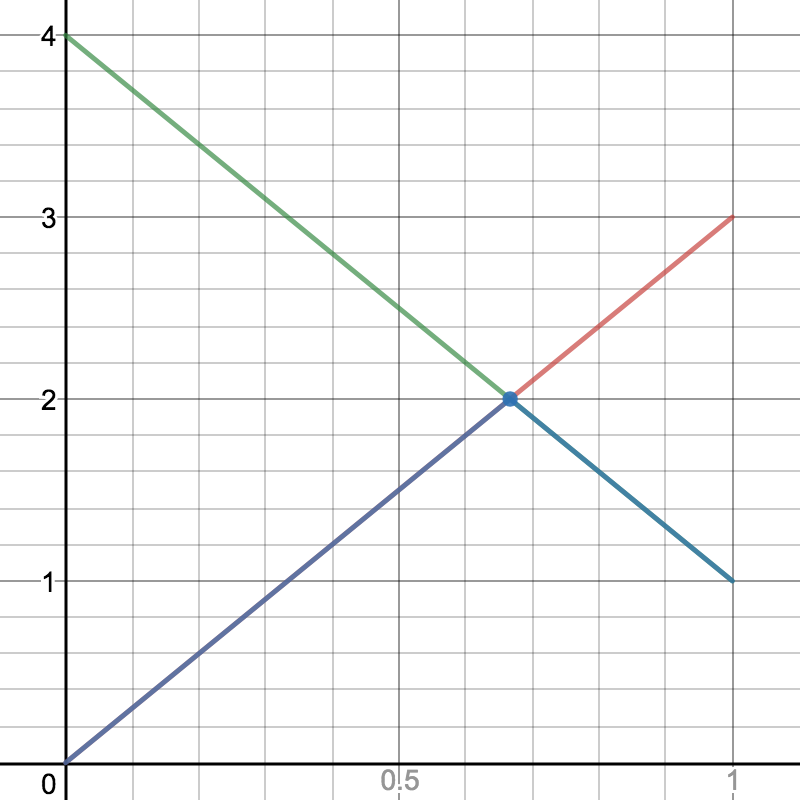
\includegraphics[width=0.8\textwidth]{20180124_07_1}
		\caption{The equilibrium is $\rnd{\frac{2}{3}, 2}$}
	\end{subfigure}
	\caption{Mixed strategy equilibrium for the row player}
\end{figure}

\begin{figure}
	\begin{subfigure}{0.49\textwidth}
		\begin{align*}
			E\sqr{\xi^{(c)}, a} & = 3\alpha + 1(1-\alpha) = 1+2\alpha  \\
			E\sqr{\xi^{(c)}, b} & = 0\alpha + 4(1-\alpha) = 4 -4\alpha
		\end{align*}
		\caption{Expected game values for the row player}
	\end{subfigure}
	\begin{subfigure}{0.49\textwidth}
		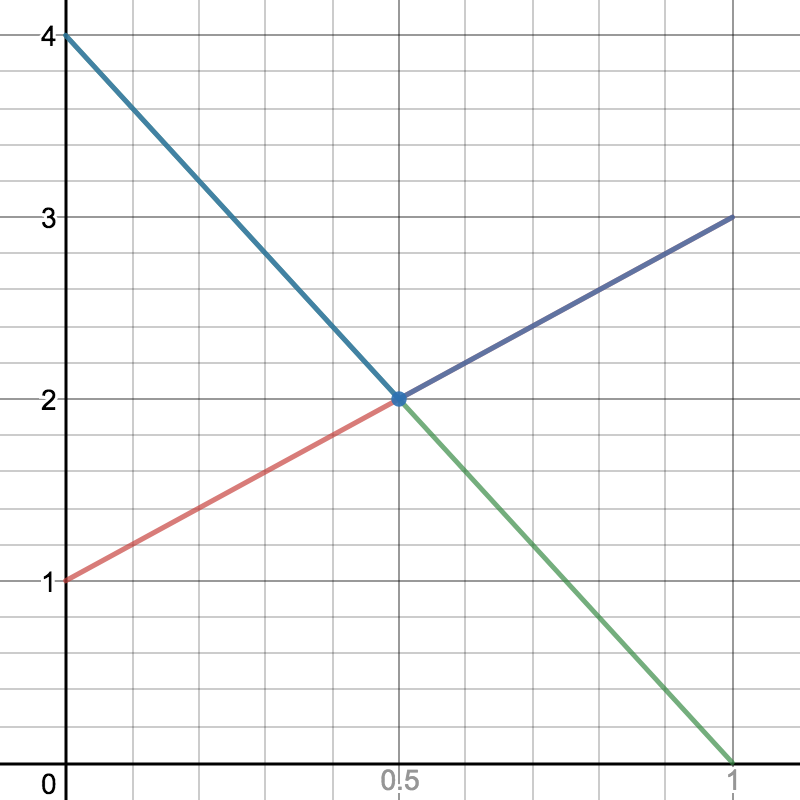
\includegraphics[width=0.8\textwidth]{20180124_07_2}
		\caption{The equilibrium is $\rnd{\frac{1}{2}, 2}$}
	\end{subfigure}
	\caption{Mixed strategy equilibrium for the column player}
\end{figure}

The mixed point of equilibrium therefore is $(\frac{2}{3}, \frac{1}{2})$.
\end{document}